\section{Abstractions}
\label{sec:abstractions}

StackwalkerAPI contains two interfaces: the Stackwalking Interface and the
Callback Interface. The stackwalking interface is used to walk the call stack,
query information about stack frames, and collect basic information about
threads. The Callback Interface is used to provide custom mechanisms for walking
a call stack. Users who operate in one of StackwalkerAPI's standard
configurations do not need to use the Callback Interface. 
    
Figure~\ref{fig:object-ownership} 1 shows the ownership hierarchy for
StackwalkerAPI's classes. Ownership is a "contains" relationship; if one class
owns another, then instances of the owner class maintain an exclusive instance
of the other. For example, in Figure~\ref{fig:object-ownership} the each Walker
instance contains exactly one instance of a ProcessState object.  No other
instance of Walker uses that instance of ProcessState.  

This remainder of this
section briefly describes the six classes that make up StackwalkerAPI's two
interfaces. For more details, see the class descriptions in
Section~\ref{sec:API}.

\begin{figure}
\centering
    \tikzstyle{class} = [rectangle, draw, rounded corners]
    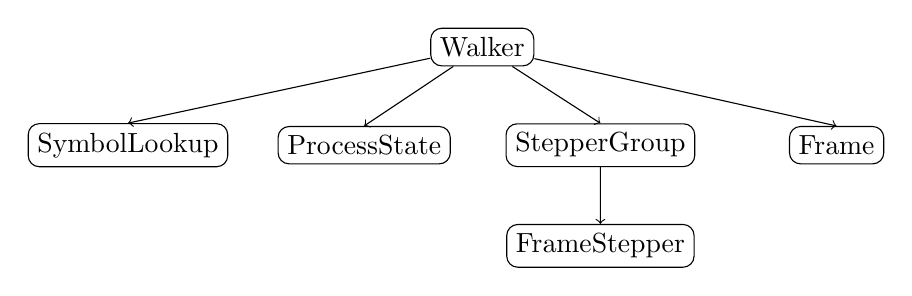
\begin{tikzpicture}[
        level distance=1cm, 
        growth parent anchor=south,
        child anchor=north,
        sibling distance=3cm
    ]

    \node [class] (Walker) {Walker} [->]
    child {
        node [class] (SymbolLookup) {SymbolLookup}
    }
    child {
        node [class] (ProcessState) {ProcessState}
    }
    child {
        node [class] (StepperGroup) {StepperGroup}
        child {
            node [class] (FrameStepper) {FrameStepper}    
        }
    }
    child {
        node [class] (Frame) {Frame}
    }
    ;
    
\end{tikzpicture}
\caption{Object Ownership}
\label{fig:object-ownership}

\end{figure}



\subsection{Stackwalking Interface}
\begin{description}
    \item [Walker] The Walker class is the top-level class used for collecting
        stackwalks. It provides a simple interface for requesting a stackwalk.
        Each Walker object is associated with one process, but may walk the call
        stacks of multiple threads within that process.
    \item [Frame] A call stack is returned as a vector of Frame objects, where
        each Frame object represents a stack frame. It can provide information
        about the stack frame and basic information about the function, signal
        handler or other mechanism that created it. Users can request
        information such as the symbolic name associated with the Frame object,
        and values of its saved registers. 
\end{description}

\subsection{Callback Interface}
StackwalkerAPI includes default implementations of the Callback Interface on
each of its supported platforms. These default implementations allow
StackwalkerAPI to work "out of the box" in a standard configuration on each
platform. Users can port StackwalkerAPI to new platforms or customize its call
stack walking behavior by implementing their own versions of the classes in the
Callback Interface.

\begin{description}
\item [FrameStepper] A FrameStepper object describes how to walk through a
    single type of stack frame. Users can provide an implementation of this
    interface that allows StackwalkerAPI to walk through new types of stack
    frames. For example, the DyninstAPI uses this interface to extend
    StackwalkerAPI to allow it to walk through stack frames created by
    instrumentation code.

\item [StepperGroup] A StepperGroup is a collection of FrameStepper objects and
    criteria that describes when to use each type of FrameStepper. These
    criteria are based on simple address ranges in the code space of the target
    process. In the above example with DyninstAPI, it would be the job of the
    StepperGroup to identify a stack frame as belonging to instrumentation code
    and use the instrumentation FrameStepper to walk through it.

\item [ProcessState] A ProcessState interface describes how to access data in
    the target process. To walk a call stack, StackwalkerAPI needs to access
    both registers and memory in the target process; ProcessState provides an
    interface that StackwalkerAPI can use to access that information.
    StackwalkerAPI includes two default implementation of ProcessState for each
    platform: one to collect a first party stackwalk in the current process, and
    one that uses a debugger interface to collect a third party stackwalk in
    another process.

\item [SymbolLookup] The SymbolLookup interface is used to associate a symbolic
    name with a stack frame. A stackwalk returns a collection of addresses in
    the code space of a binary. This class uses the binary's symbol table to map
    those addresses into symbolic names. A default implementation of this class,
    which uses the DynSymtab package, is provided with StackwalkerAPI. A user
    could, for example, use this interface to allow StackwalkerAPI to use libelf
    to look up symbol names instead.
\end{description}
